% Free-fall lab report. Build from ../ with `make` (runs the analysis first).
% Rules: ../../report-rules.md (general), ../report-rules.md (free fall).
% Limits: 10 pages excluding cover + appendices; 10 numbered formulas excluding (1)-(2).
\documentclass[10pt,a4paper]{article}

\usepackage[a4paper,margin=2cm]{geometry}
\usepackage{amsmath}
\usepackage{graphicx}
\usepackage{tikz}
\usepackage{xcolor}
\usepackage[labelsep=colon,font=small]{caption}
\usepackage{fontspec}
% LuaLaTeX + babel instead of XeLaTeX + polyglossia (2026-10-28): under XeTeX's bidi,
% \textcolor leaked to whole RTL lines; luacolor colours per character.
\usepackage{luacolor}
\usepackage[bidi=basic, layout=lists.tabular, main=hebrew, english]{babel}
% Times New Roman (macOS system font, has Hebrew). Frank Ruehl CLM from TeX Live was
% tried first: its digits are heavy and read as bold next to the body text.
\babelfont[hebrew]{rm}{Times New Roman}
\newcommand{\textenglish}[1]{\foreignlanguage{english}{#1}}

% Paragraphs: no first-line indent, small gap between paragraphs (Word-like, as in the guide).
\setlength{\parindent}{0pt}
\setlength{\parskip}{4pt plus 1pt}

% Content added by Claude beyond the Doc (user, 2026-10-28). Blue until the pair reviews it;
% turn black (drop the macro) once approved. Must not survive into the submitted PDF either.
\newcommand{\added}[1]{\textcolor{blue}{#1}}

% Visible placeholder for anything not written yet. Must not survive into the submitted PDF.
\newcommand{\TODO}[1]{\textcolor{red}{[#1]}}
% Units after a value in math mode: $\LinG\U{cm/s^2}$
\newcommand{\U}[1]{\,\mathrm{#1}}

% Generated by analysis/analysis.py -- do not edit by hand.
% Values are in math mode; units are written in the report text.
\newcommand{\LinAZero}{0.867 \pm 0.061}
\newcommand{\LinAZeroRel}{7.1\%}
\newcommand{\LinAOne}{501.25 \pm 0.81}
\newcommand{\LinAOneRel}{0.16\%}
\newcommand{\LinChi}{3.5}
\newcommand{\LinP}{5.3 \cdot 10^{-4}}
\newcommand{\LinG}{1002.5 \pm 1.6}
\newcommand{\LinGRel}{0.16\%}
\newcommand{\LinNsigma}{2.1}
\newcommand{\ParAZero}{-0.07 \pm 0.10}
\newcommand{\ParAZeroRel}{140\%}
\newcommand{\ParAOne}{8.34 \pm 0.87}
\newcommand{\ParAOneRel}{10\%}
\newcommand{\ParATwo}{485.0 \pm 1.7}
\newcommand{\ParATwoRel}{0.35\%}
\newcommand{\ParChi}{0.28}
\newcommand{\ParP}{0.96}
\newcommand{\ParG}{969.9 \pm 3.4}
\newcommand{\ParGRel}{0.35\%}
\newcommand{\ParNsigma}{1.0}
\newcommand{\DelayMs}{8.6}
\newcommand{\DelayDistMm}{0.36}
\newcommand{\NsigmaFits}{8.6}
\newcommand{\GTheo}{981 \pm 10}
\newcommand{\HRes}{0.1}
\newcommand{\TRes}{10^{-5}}

% Cover-page details. Fill these in; everything else on the cover is fixed.
\newcommand{\ExperimentName}{נפילה חופשית}
\newcommand{\ExperimentPart}{\TODO{חלק}}
\newcommand{\InstructorName}{\TODO{שם מלא של המדריך}}
\newcommand{\ExperimentDate}{19.10.2026}
\newcommand{\SubmissionDate}{\TODO{תאריך הגשה}}
\newcommand{\StudentOneFirst}{איתמר}
\newcommand{\StudentOneLast}{אביגדורי}
\newcommand{\StudentOneID}{\TODO{ת.ז.}}
\newcommand{\StudentTwoFirst}{ליאור}
\newcommand{\StudentTwoLast}{ביינהורן}
\newcommand{\StudentTwoID}{\TODO{ת.ז.}}
\newcommand{\StudyTrack}{\TODO{מסלול}}
\newcommand{\LabGroup}{\TODO{קבוצה}}
\newcommand{\SubGroup}{\TODO{תת קבוצה}}
\newcommand{\Station}{\TODO{עמדה}}


\begin{document}
% Cover page, laid out after ../../cover-page-template.docx (Moodle template).
% Not counted in the page limit and not numbered.
\begin{titlepage}
\thispagestyle{empty}
\noindent
\fbox{\begin{minipage}[t][3.2cm]{0.52\textwidth}
  \vspace{0.4cm}
  \Large\textbf{דו"ח מסכם בניסוי: \ExperimentName}\\[0.6cm]
  \textbf{חלק: \ExperimentPart}
\end{minipage}}
\hfill
\fbox{\begin{minipage}[t][3.2cm]{0.36\textwidth}
  \vspace{0.3cm}
  שם הבודק: \rule{2.8cm}{0.4pt}\\[0.35cm]
  תאריך הבדיקה: \rule{2.4cm}{0.4pt}\\[0.35cm]
  ציון הדו"ח: \quad I \rule{1cm}{0.4pt}\\[0.2cm]
  \hspace*{1.95cm} II \rule{1cm}{0.4pt}
\end{minipage}}

\vspace{1.5cm}
\noindent שם מדריך הניסוי (שם מלא): \InstructorName\\[0.5cm]
תאריך ביצוע הניסוי: \ExperimentDate\\[0.5cm]
תאריך הגשת הדו"ח: \SubmissionDate

\vspace{1.2cm}
\noindent\textbf{הדו"ח מוגש על ידי:}

\vspace{0.6cm}
\noindent
\begin{tabular}{c@{\hspace{0.6cm}}c@{\hspace{0.6cm}}c@{\hspace{0.6cm}}c}
 & שם פרטי & משפחה & ת.ז. \\ \hline
I & \StudentOneFirst & \StudentOneLast & \StudentOneID \\[0.3cm]
II & \StudentTwoFirst & \StudentTwoLast & \StudentTwoID \\
\end{tabular}

\vspace{1cm}
\noindent
\begin{tabular}{cccc}
\StudyTrack & \LabGroup & \SubGroup & \Station \\ \hline
מסלול הלימוד & מס' קבוצת המעבדה & תת קבוצה & מספר עמדה \\
\end{tabular}

\vspace{1.5cm}
\noindent\rule{\textwidth}{1.2pt}

\vspace{0.4cm}
\noindent\underline{\textbf{הערות הבודק לנושאים לקויים בדו"ח:}}
\end{titlepage}

\setcounter{page}{1}

\section*{מטרות הניסוי}
\begin{enumerate}
% src: GOAL-01
  \item אימות נוסחת הנפילה החופשית\added{: בדיקה שתאוצת הכובד המחולצת מהמדידות תואמת לערך התיאורטי בטווח הטעות המקובל ($N_\sigma \le 3$), ושהיא נמדדת בדיוק של שגיאה יחסית הקטנה מ-5\%}.
% src: GOAL-02
  \item התנסות בכלים סטטיסטיים \added{לעיבוד המדידות: הערכת שגיאות ושקלולן, התאמת מודל למדידות ובחינת טיב ההתאמה}.
\end{enumerate}

\section*{רקע תיאורטי}
% Verbatim from ../theory-background-format.docx (staff file from Moodle).
% src: THEO-01 THEO-02
נפילה חופשית הינה התנועה הנוצרת בעת שחרור גוף ממנוחה באוויר, מה שמוביל לנפילת הגוף עקב השפעת כוח המשיכה של כדור הארץ בלבד. כלומר, אינו מושפע מגורמים חיצוניים כדוגמת רוח והתנגדות האוויר.

% src: THEO-03 THEO-04
מהגדרת הנפילה החופשית, נסיק כי הכוח היחיד הפועל על הגוף הינו כוח הכבידה, ולכן התאוצה של הגוף הינה תאוצת הכובד. נהוג לסמן את תאוצת הכובד באות $g$, וערכה על פני השטח של כדור הארץ הוא בקירוב:
% src: THEO-05
\[ g_{\mathrm{theoretical}} = \GTheo\U{cm/s^2} \]
% src: THEO-06
(לפי תדריך הניסוי).

% src: THEO-07 THEO-08
במהלך הניסוי הנוכחי נגדיר את כיוון התנועה החיובי במערכת הצירים כציר האנכי הפונה מטה. מכיוון שתאוצת הגוף היא קבועה (בקירוב), נשתמש בנוסחת התנועה בתאוצה קבועה:
% src: THEO-09
\begin{equation}\label{eq:motion}
h = h_0 + v_0 t + \frac{1}{2} g t^2
\end{equation}
% src: THEO-10 THEO-11 THEO-12 THEO-13
האות $h$ מייצגת את מיקום הגוף ו-$t$ מייצגת זמן. מיקום הגוף בזמן $t=0$ ייוצג על ידי $h_0$, המהירות ההתחלתית תסומן ב-$v_0$ ותאוצת הגוף תסומן ב-$g$. כיוון שמדובר בנפילה חופשית, נצא מנקודת הנחה שהמהירות ההתחלתית תהיה אפס, כלומר $v_0 = 0\U{cm/s}$. לכן, לאחר בחירת הגובה ההתחלתי $h_0 = 0$ כראשית הצירים, והצבתו במשוואה \eqref{eq:motion}, נקבל את הנוסחה הבאה:
% src: THEO-14
\begin{equation}\label{eq:freefall}
h = \frac{1}{2} g t^2
\end{equation}

\section*{מהלך הניסוי}
% Equipment list and setup text sit beside the schematic they refer to (user, 2026-10-28).
% RTL: the first minipage lands on the right.
\noindent
\begin{minipage}[t]{0.52\textwidth}
\subsection*{רשימת ציוד}
% Numbers here match the labels in the setup figure (general rules 4.3.2).
% Items 5-7 are in the Doc's figure (SETUP-01) but not in its equipment list.
% Item 9 (optical gate) is not drawn in the figure; it starts the timing (DISC-36, briefing), user decision 2026-10-29.
\begin{enumerate}
% src: EQUIP-07
  \item אלקטרומגנט, המשמש כיחידת שחרור לכדור.
% src: EQUIP-01
  \item כדור מתכת.
% src: EQUIP-02 EQUIP-03
  \item מעמד: עמוד מדורג המשמש כסרגל, ברזולוציה של $\HRes\U{cm}$.
% src: EQUIP-06
  \item לוחית מתכת וחיישן פיזואלקטרי, על משטח שגובהו מתכוונן.
% src: SETUP-01
  \item תופסן לנעילת המשטח על המעמד.
% src: SETUP-01
  \item בסיס המעמד.
% src: SETUP-01
  \item כבלי אות.
% src: EQUIP-04
  \item מחשב ותוכנה למדידת זמן הנפילה, ברזולוציה של $\TRes\U{s}$.
% src: EQUIP-05
  \item שער אופטי אינפרא-אדום\added{, המפעיל את מדידת הזמן (סומן באיור בכחול)}.
\end{enumerate}
\subsection*{מערכת הניסוי}
% src: SETUP-02
מערכת הניסוי מתוארת באיור~\ref{fig:setup}. היא מורכבת מעמוד מדורג המשמש כסרגל גובה (3), מאלקטרומגנט (1) המשחרר את הכדור (2) לפי פקודה, וממשטח בגובה מתכוונן (4) שעליו חיישן פיזואלקטרי.
% src: SETUP-03
האלקטרומגנט והחיישן הפיזואלקטרי מחוברים בכבלי אות (7) למחשב (8)\added{. מדידת הזמן מתחילה כאשר הכדור חוצה את קרן השער האופטי (9), ומסתיימת כאשר הוא פוגע בחיישן}.
% src: SETUP-01
גובה הנפילה $h$ מוגדר כמרחק בין תחתית הכדור לפני השחרור לבין משטח החיישן.
\end{minipage}\hfill
\begin{minipage}[t]{0.44\textwidth}
  \vspace{0pt}
  \centering
% src: SETUP-01
  % Optical gate (item 9) is not in the original drawing; drawn on top in blue for review
  % (user, 2026-10-29). Coordinates are fractions of the image: x from the left, y from the bottom.
  % LTR block: under RTL (babel bidi) the picture's x axis is mirrored.
  \begin{otherlanguage}{english}
  \begin{tikzpicture}
    \node[inner sep=0, anchor=south west] (img) {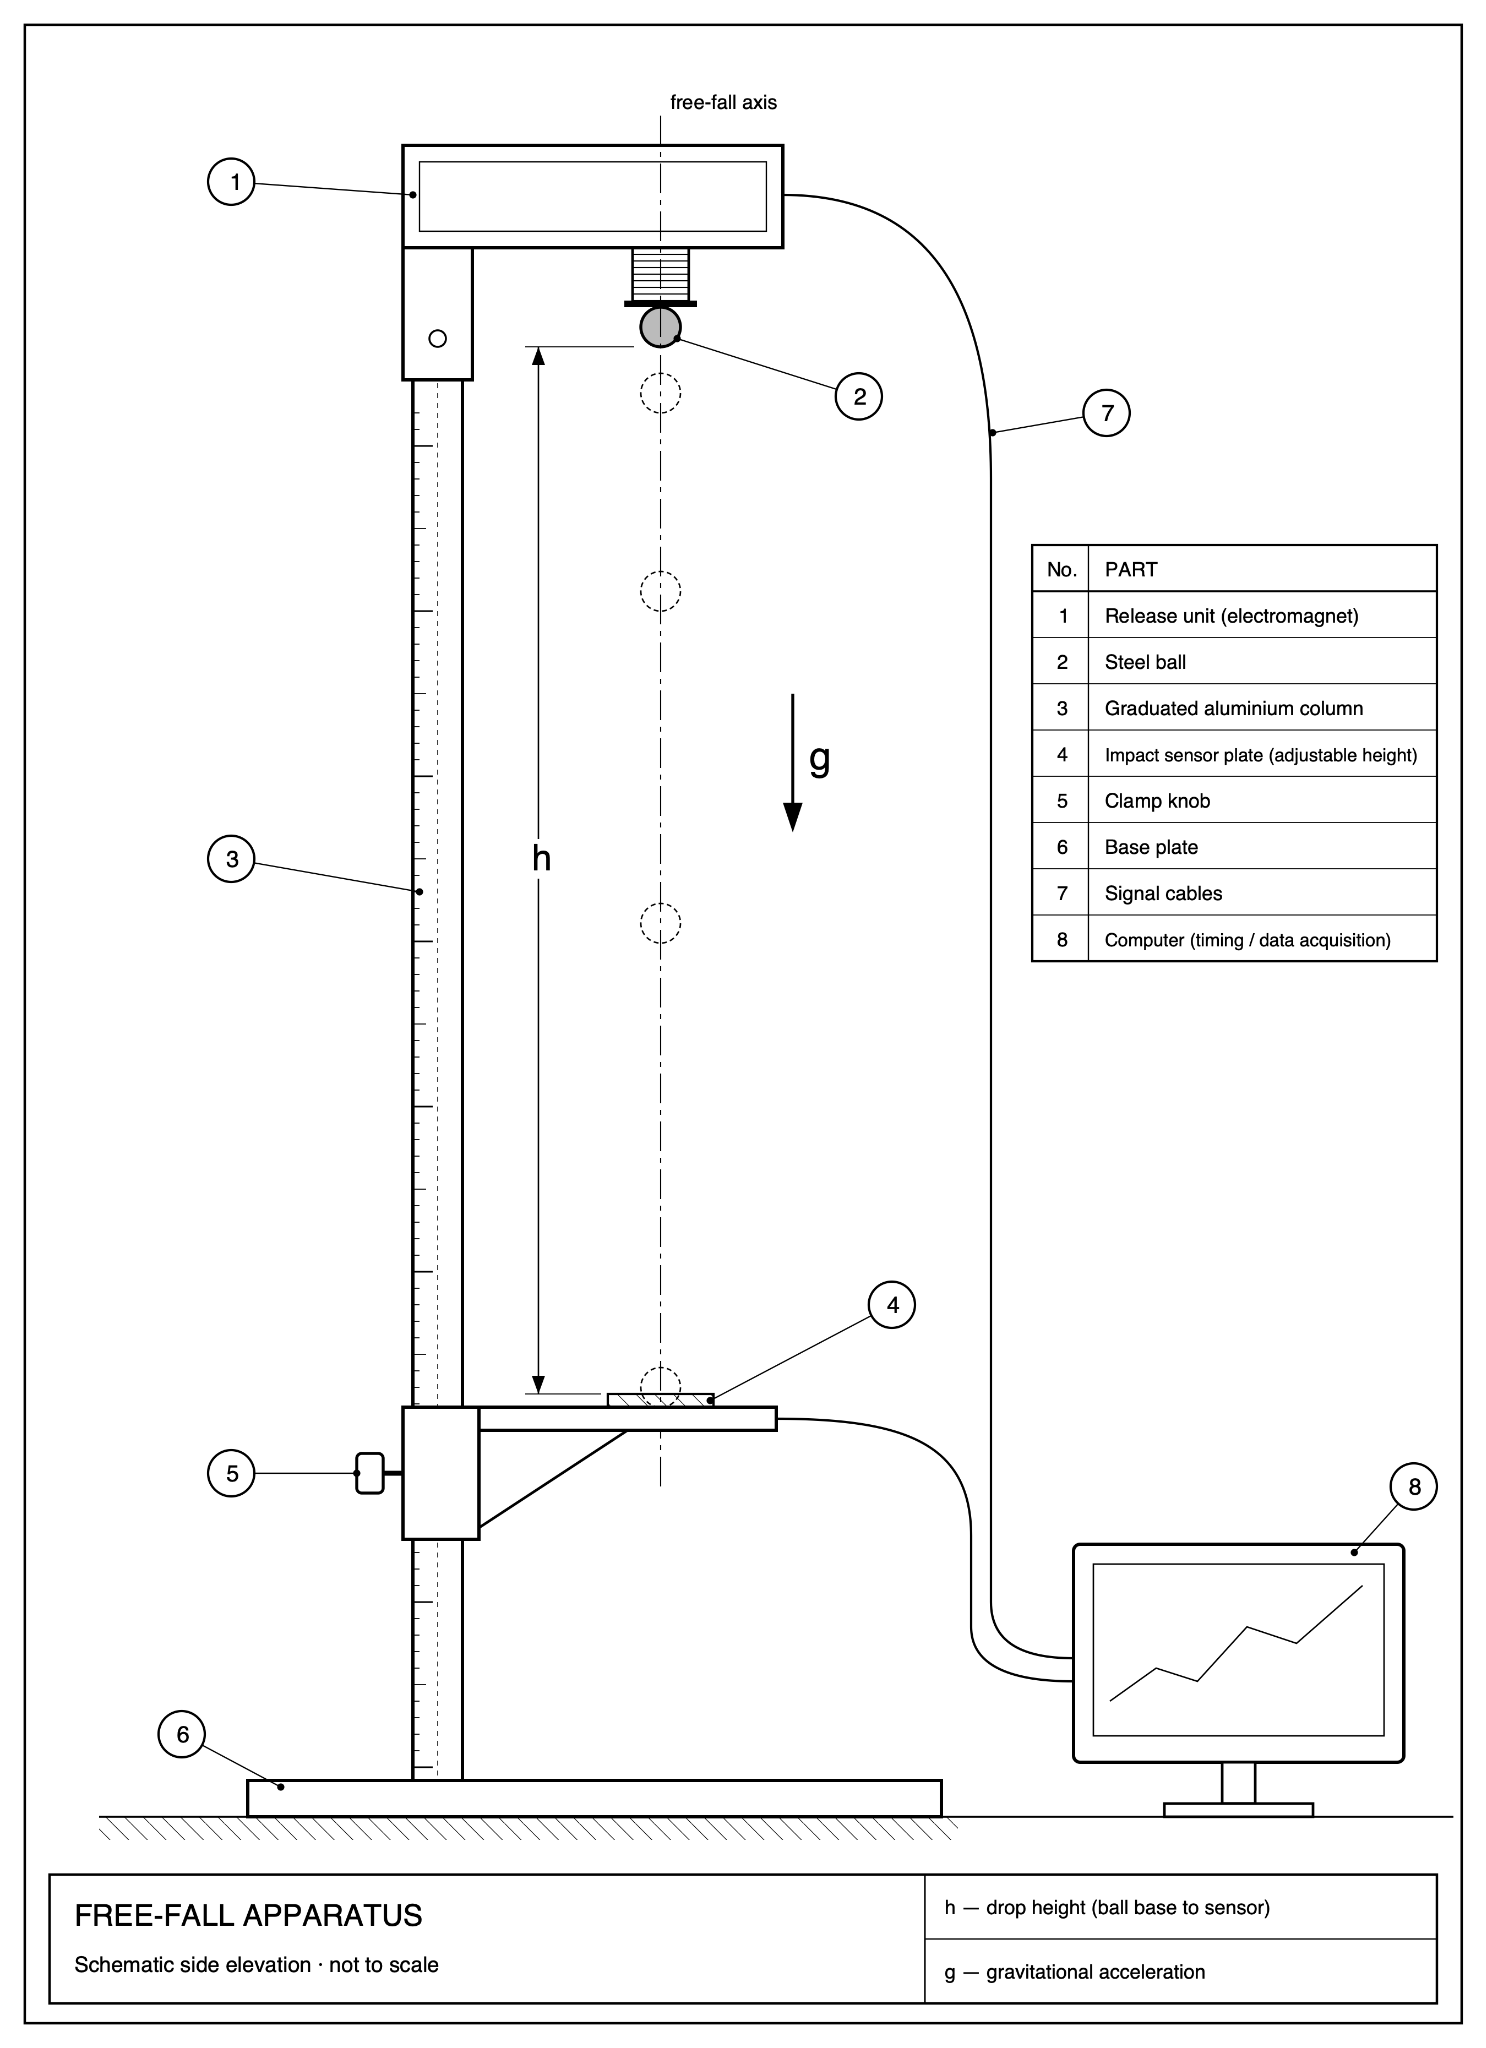
\includegraphics[width=\textwidth]{figures/setup.png}};
    \begin{scope}[x={(img.south east)}, y={(img.north west)}, blue, line width=0.5pt]
      \draw[fill=blue!15] (0.395,0.758) rectangle (0.415,0.772);   % emitter
      \draw[fill=blue!15] (0.475,0.758) rectangle (0.495,0.772);   % receiver
      \draw[dashed] (0.415,0.765) -- (0.475,0.765);                % beam across the fall axis
      \draw (0.495,0.765) -- (0.545,0.765);                        % leader
      \node[draw, circle, inner sep=0.6pt, font=\tiny] at (0.565,0.765) {9};
    \end{scope}
  \end{tikzpicture}
  \end{otherlanguage}
  \captionof{figure}{\added{תרשים סכמטי של מערכת הניסוי. המספור תואם לרשימת הציוד.}}
  \label{fig:setup}
\end{minipage}

\subsection*{שלבי הניסוי}
\begin{enumerate}
% src: PROC-01 PROC-02
  \item בדיקת המערכת: המערכת הוצבה על שולחן ובוצעה מדידת ניסיון לבדיקת תקינותה. במהלך הבדיקה בוצעו כ-3 מדידות מאותו הגובה, כדי לוודא שהתוצאות קרובות זו לזו.
% src: PROC-03
  \item ביצוע מדידה בודדת:
  \begin{enumerate}
% src: PROC-04
    \item המשטח (4) כוון לגובה הרצוי לפי הסרגל (3).
% src: PROC-05
    \item המשטח ננעל במקומו באמצעות התופסן (5), כדי שלא יזוז או ייפול בין המדידות.
% src: PROC-06
    \item האלקטרומגנט (1) הופעל דרך תוכנת המחשב (8).
% src: PROC-07
    \item הכדור (2) הוצמד לאלקטרומגנט.
% src: PROC-08 PROC-09
    \item שחרור הכדור הופעל דרך תוכנת המחשב. התוכנה תיעדה אוטומטית את משך הנפילה, \added{מהרגע שבו הכדור חצה את קרן השער האופטי (9)} ועד רגע הפגיעה במשטח.
  \end{enumerate}
% src: PROC-10
  \item בחירת גבהים: משך הנפילה נמדד מעשרה גבהים, בסנטימטרים: $10, 15, 20, 30, 40, 45, 50, 60, 70, 80$.
% src: PROC-11 PROC-12
  \item בכל גובה בוצעו 10 מדידות כמתואר בסעיף 2, והגובה הנמדד תועד בתוכנה.
% src: PROC-13
  \item בסוף הניסוי יוצאו התוצאות מהתוכנה לקובץ \textenglish{Excel}.
\end{enumerate}
\TODO{נימוק לבחירת הגבהים ולמספר החזרות — חסר במסמך המשותף}

\section*{תכנון עיבוד התוצאות}
% Formula budget (free-fall rules 7): numbered here (3)-(9), 7 of 10.
% Booklet ("החוברת") formulas are cited by number; adapted ones are written and numbered.
% src: PLAN-01 PLAN-02
מטרת העיבוד היא לבחון את מודל הנפילה החופשית המתואר בנוסחה \eqref{eq:freefall}. מודל זה הוא מקרה פרטי של נוסחה \eqref{eq:motion}, המתקבל מתוך ההנחות שפורטו ברקע התיאורטי: הגוף משוחרר ממנוחה, ומיקומו ההתחלתי מוגדר כ-$h=0$.
% src: PLAN-03
המודל ייבחן בשתי התאמות: התאמה לינארית של $h$ כתלות ב-$t^2$, והתאמה פרבולית של $h$ כתלות ב-$t$.

\subsection*{הגדלים הנמדדים ושגיאותיהם}
% src: PLAN-05
לפני ביצוע ההתאמות יחושבו הגדלים הדרושים ושגיאותיהם.
% src: PLAN-06
גובה הנפילה $h$ נמדד פעם אחת בכל גובה באמצעות הסרגל, ולכן שגיאתו היא שגיאת רזולוציה, המחושבת לפי נוסחה (28) בחוברת עיבוד הנתונים תחת הנחת התפלגות אחידה בין שנתות הסרגל:
\begin{equation}\label{eq:dh}
\Delta h = \frac{h_{res}}{\sqrt{12}}
\end{equation}
כאשר $h_{res} = \HRes\U{cm}$ היא רזולוציית הסרגל.

% src: PLAN-08 PLAN-09
זמן הנפילה נמדד 10 פעמים בכל גובה, וזמן הנפילה $t$ יילקח כממוצע המדידות, כדי להקטין את השגיאה הסטטיסטית. לזמן הנפילה שני מקורות שגיאה: שגיאת רזולוציה של תוכנת המדידה, תחת הנחת התפלגות אחידה (נוסחה (28) בחוברת), ושגיאה סטטיסטית.
% src: PLAN-10
השגיאה הסטטיסטית $\Delta t_{stat}$ תחושב מסטיית התקן המדגמית של 10 המדידות, לפי נוסחאות (32) ו-(34) בחוברת.
% src: PLAN-11
השגיאה הכוללת בזמן הנפילה מתקבלת משקלול שני מקורות השגיאה לפי נוסחה (35) בחוברת:
\begin{equation}\label{eq:dt}
\Delta t = \sqrt{\Delta t_{stat}^2 + \left(\frac{t_{res}}{\sqrt{12}}\right)^2}
\end{equation}
כאשר $t_{res} = \TRes\U{s}$ היא רזולוציית תוכנת המדידה.

\subsection*{התאמה לינארית}
% src: PLAN-13 PLAN-14
להתאמה זו נדרש ריבוע זמן הנפילה $t^2$, שיחושב מהזמן הממוצע. שגיאתו היא שגיאה עקיפה, שתחושב לפי נוסחה (39) בחוברת כאשר המשתנה הישיר הוא $t$:
\begin{equation}\label{eq:dt2}
\Delta(t^2) = 2t\,\Delta t
\end{equation}

% src: PLAN-04 PLAN-15
הגדלים ושגיאותיהם יוזנו למחברת ה-\textenglish{Colab} של הקורס, ותותאם להם \added{בשיטת \textenglish{ODR}} פונקציה לינארית:
\begin{equation}\label{eq:linfit}
y = a_0 + a_1 x
\end{equation}
כאשר $x = t^2$ ו-$y = h$.
% src: PLAN-24 PLAN-25
לפי נוסחה \eqref{eq:freefall}, הפרמטר $a_1$ מייצג את $\frac{1}{2}g$, והאיבר החופשי $a_0$ צפוי להתאפס. תאוצת הכובד ושגיאתה העקיפה יחולצו מההתאמה לפי:
\begin{equation}\label{eq:glin}
g = 2a_1 \pm 2\Delta a_1
\end{equation}

\subsection*{התאמה פרבולית}
% src: PLAN-28 PLAN-29
בהתאמה השנייה תותאם לנתונים פונקציה פרבולית לפי נוסחה \eqref{eq:motion}:
\begin{equation}\label{eq:parfit}
y = a_0 + a_1 x + a_2 x^2
\end{equation}
כאשר $x = t$ ו-$y = h$.
% src: PLAN-30 PLAN-31
הגובה, הזמן ושגיאותיהם הם אלו שיחושבו לפי נוסחאות \eqref{eq:dh} ו-\eqref{eq:dt}. בהתאמה זו אין צורך בשגיאה עקיפה, מכיוון ש-$t$ ו-$h$ נמדדים ישירות.
% src: PLAN-43 PLAN-44 PLAN-45 PLAN-46
לפי נוסחה \eqref{eq:motion}, הפרמטר $a_0$ מייצג את הגובה ההתחלתי ו-$a_1$ את המהירות ההתחלתית, ולכן שניהם צפויים להתאפס. הפרמטר $a_2$ מייצג מחצית מהתאוצה, ולכן צפוי להיות $\frac{1}{2}g$.
% added (not in the Doc): briefing formula (7); report-gaps.md "parabolic fit has no g formula".
\added{תאוצת הכובד ושגיאתה העקיפה יחולצו מההתאמה לפי:}
{\color{blue}
\begin{equation}\label{eq:gpar}
g = 2a_2 \pm 2\Delta a_2
\end{equation}}

\subsection*{בחינת ההתאמות}
% src: PLAN-16 PLAN-17 PLAN-18 PLAN-19 PLAN-33 PLAN-34 PLAN-35 PLAN-36 PLAN-37 PLAN-38 PLAN-55 PLAN-56
מכל התאמה יתקבלו הפרמטרים ושגיאותיהם, ולכל פרמטר תחושב השגיאה היחסית, באחוזים, לפי נוסחה (25) בחוברת. השגיאה היחסית מבטאת את גודל השגיאה ביחס לערך הנמדד. בקורס זה שגיאה יחסית הקטנה מ-5\% נחשבת קטנה.
% added (not in the Doc): the briefing's test for parameters expected to vanish (free-fall rules 6).
\added{פרמטר שצפוי להתאפס ייחשב תואם לצפי אם שגיאתו היחסית גדולה מ-50\% או שווה לה, לפי תדריך הניסוי.}
% src: PLAN-47
איכות כל התאמה תיבחן באמצעות המדדים הבאים:
\begin{itemize}
% src: PLAN-20 PLAN-21 PLAN-39 PLAN-40 PLAN-48 PLAN-49
  \item חי בריבוע מצומצם, $\chi^2_{red}$ (נוסחה (50) בחוברת), המבטא את מידת ההתאמה בין נקודות המדידה לגרף ההתאמה. בהתאמה תקינה צפוי ערך קרוב ל-1.
% src: PLAN-22 PLAN-23 PLAN-41 PLAN-42 PLAN-50 PLAN-51
  \item \textenglish{p-value}: ההסתברות לקבל ערך $\chi^2_{red}$ גדול מזה שהתקבל או שווה לו, בהנחה שהמודל מתאר את המערכת. \added{הוא מחושב מהתפלגות חי בריבוע, לפי $\chi^2$ ומספר דרגות החופש $N-K$ שבנוסחה (50) בחוברת.} ערכים תקינים הם בתחום $0.05 \le p \le 0.95$.
% src: PLAN-57
  \item גרף השארים, שבו ייבדק שפיזור הנקודות סביב קו האפס אקראי וללא מגמה.
\end{itemize}
% src: PLAN-26 PLAN-27 PLAN-52 PLAN-53 PLAN-54
תאוצת הכובד שתחולץ מכל התאמה תושווה לערך התיאורטי $g = \GTheo\U{cm/s^2}$ באמצעות מדד $N_\sigma$ (נוסחה (51) בחוברת). שתי התוצאות נחשבות תואמות אם $N_\sigma \le 3$.

\section*{תוצאות}
\subsection*{התאמה לינארית}
\begin{figure}[h]
  \centering
  % RTL: the first minipage lands on the right, so the fit (read first) comes first.
  \begin{minipage}[t]{0.48\textwidth}
    \centering
% src: RES-02
    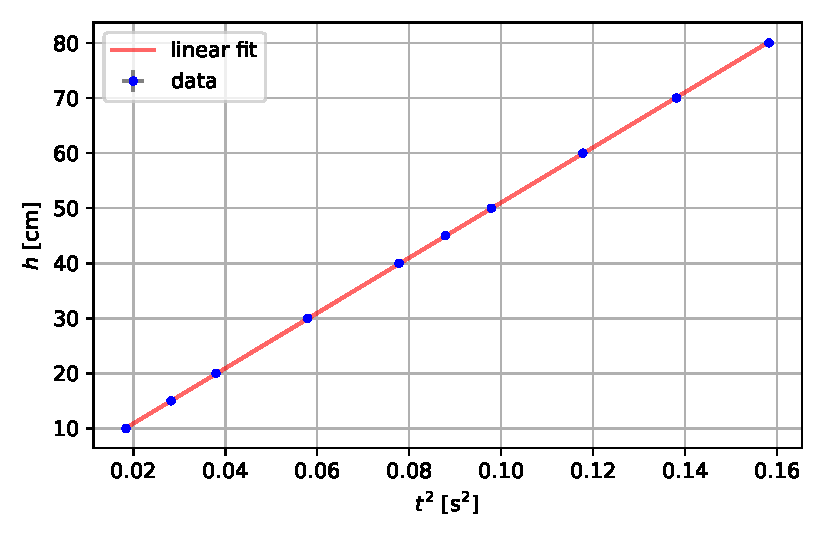
\includegraphics[width=\textwidth]{figures/lin_fit.pdf}
    \caption{\added{גובה הנפילה $h$ בסנטימטרים כתלות בריבוע זמן הנפילה $t^2$ בשניות בריבוע, וההתאמה הלינארית לפי נוסחה \eqref{eq:linfit}.}}
    \label{fig:lin-fit}
  \end{minipage}\hfill
  \begin{minipage}[t]{0.48\textwidth}
    \centering
% src: RES-02
    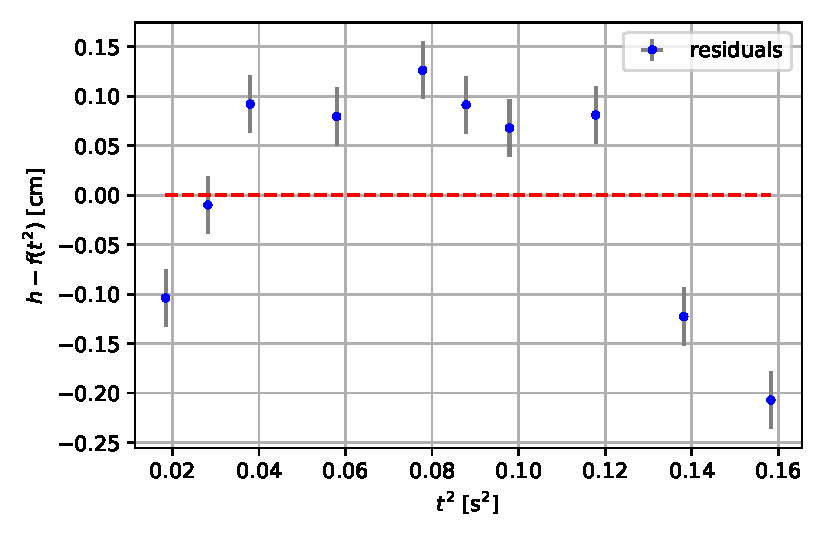
\includegraphics[width=\textwidth]{figures/lin_res.pdf}
    \caption{\added{גרף השארים של ההתאמה הלינארית: ההפרש בין גובה הנפילה הנמדד לבין ערך פונקציית ההתאמה, בסנטימטרים, כתלות ב-$t^2$ בשניות בריבוע. צלבי השגיאה מציגים את $\Delta h$ בלבד.}}
    \label{fig:lin-res}
  \end{minipage}
\end{figure}
% src: RES-01 RES-06 RES-18
גרף ההתאמה הלינארית וגרף השארים שלה מוצגים באיור~\ref{fig:lin-fit} ובאיור~\ref{fig:lin-res}. פרמטרי שתי ההתאמות ומדדיהן מרוכזים בטבלה~\ref{tab:results}.
% src: RES-03
בגרף ההתאמה, נקודות המדידה נמצאות על קו ההתאמה או בסמוך מאוד אליו.
% src: RES-04
בגרף השארים, הנקודות בקצוות התחום (ערכי $t^2$ קטנים וגדולים) נמצאות מתחת לקו האפס, והנקודות במרכזו נמצאות מעליו. בשארים ניכרת מגמה פרבולית, ולא פיזור אקראי.
% src: RES-05
עם זאת, \added{כל} השארים נמצאים במרחק של \added{פחות מפי 3 משגיאתם בהתאמה} מקו האפס.
% added (not in the Doc): parameters vs expectation and meaning of the statistics (guide; checklist "Results").
\added{בטבלה~\ref{tab:results} ניתן לראות כי שגיאתו היחסית של האיבר החופשי $a_0$ קטנה מ-50\%, וכי ה-\textenglish{p-value} קטן מ-0.05. עבור תאוצת הכובד שחולצה התקבל $N_\sigma$ הקטן מ-3, ושגיאתה היחסית קטנה מ-5\%.}

\subsection*{התאמה פרבולית}
\begin{figure}[h]
  \centering
  % RTL: the first minipage lands on the right, so the fit (read first) comes first.
  \begin{minipage}[t]{0.48\textwidth}
    \centering
% src: RES-14
    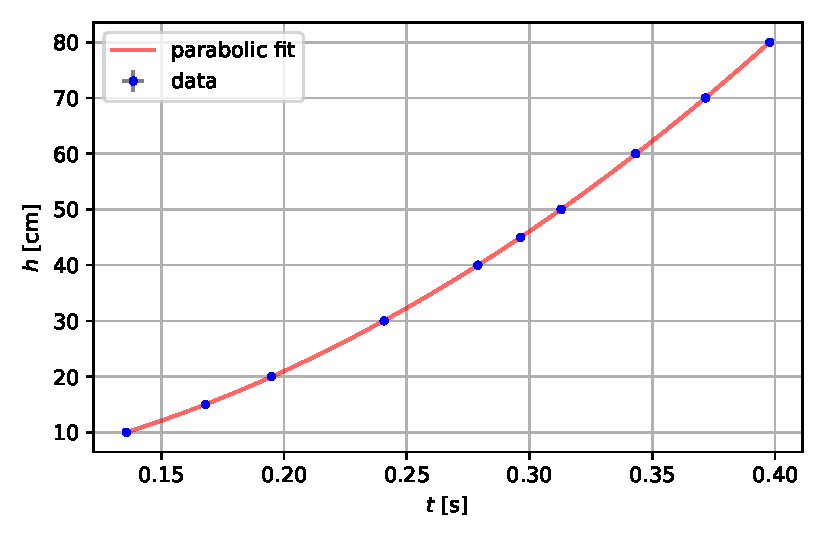
\includegraphics[width=\textwidth]{figures/par_fit.pdf}
    \caption{\added{גובה הנפילה $h$ בסנטימטרים כתלות בזמן הנפילה $t$ בשניות, וההתאמה הפרבולית לפי נוסחה \eqref{eq:parfit}.}}
    \label{fig:par-fit}
  \end{minipage}\hfill
  \begin{minipage}[t]{0.48\textwidth}
    \centering
% src: RES-14
    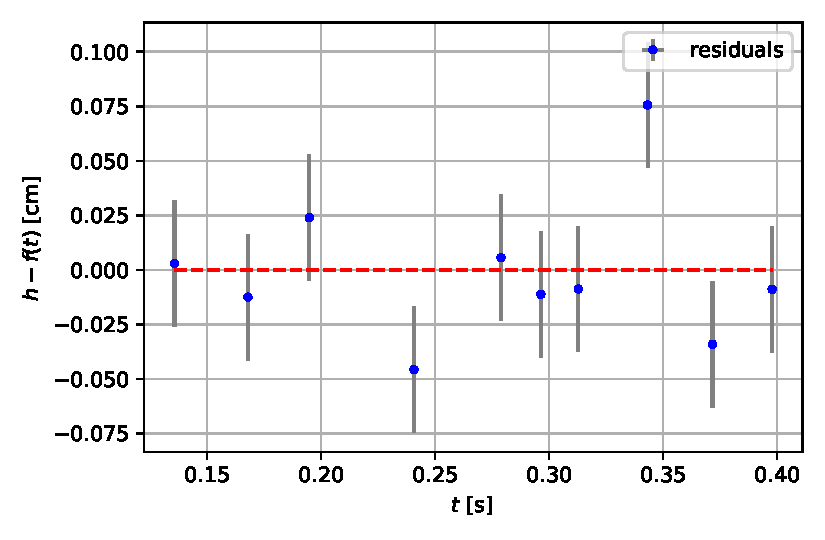
\includegraphics[width=\textwidth]{figures/par_res.pdf}
    \caption{\added{גרף השארים של ההתאמה הפרבולית: ההפרש בין גובה הנפילה הנמדד לבין ערך פונקציית ההתאמה, בסנטימטרים, כתלות ב-$t$ בשניות. צלבי השגיאה מציגים את $\Delta h$ בלבד.}}
    \label{fig:par-res}
  \end{minipage}
\end{figure}
% src: RES-13
גרף ההתאמה הפרבולית וגרף השארים שלה מוצגים באיור~\ref{fig:par-fit} ובאיור~\ref{fig:par-res}.
% src: RES-15
בגרף ההתאמה, נקודות המדידה נמצאות על קו ההתאמה או בסמוך מאוד אליו.
% src: RES-16 RES-17
בגרף השארים, הנקודות מפוזרות באקראי סביב קו האפס, וסכום השארים קרוב לאפס. רוב צלבי השגיאה חוצים את קו האפס, \added{וכל השארים} נמצאים במרחק של \added{פחות מפי 3 משגיאתם} ממנו.
% added (not in the Doc): parameters vs expectation and meaning of the statistics (guide; checklist "Results").
\added{בטבלה~\ref{tab:results} ניתן לראות כי שגיאתו היחסית של האיבר החופשי $a_0$ גדולה מ-50\%, ושל הפרמטר $a_1$ קטנה מ-50\%. ה-\textenglish{p-value} גדול מ-0.95. עבור תאוצת הכובד שחולצה התקבל $N_\sigma$ הקטן מ-3, ושגיאתה היחסית קטנה מ-5\%.}

\begin{table}[h]
  \centering
  \renewcommand{\arraystretch}{1.3}
  \begin{tabular}{|c|c|c|c|c|}
    \hline
     & \multicolumn{2}{c|}{התאמה לינארית} & \multicolumn{2}{c|}{התאמה פרבולית} \\
    \cline{2-5}
     & ערך & שגיאה יחסית & ערך & שגיאה יחסית \\
    \hline
    $a_0$ & $\LinAZero\U{cm}$ & $\LinAZeroRel$ & $\ParAZero\U{cm}$ & $\ParAZeroRel$ \\ % src: RES-07 RES-19
    \hline
    $a_1$ & $\LinAOne\U{cm/s^2}$ & $\LinAOneRel$ & $\ParAOne\U{cm/s}$ & $\ParAOneRel$ \\ % src: RES-08 RES-20
    \hline
    $a_2$ & -- & -- & $\ParATwo\U{cm/s^2}$ & $\ParATwoRel$ \\ % src: RES-21
    \hline
    $g$ & $\LinG\U{cm/s^2}$ & $\LinGRel$ & $\ParG\U{cm/s^2}$ & $\ParGRel$ \\ % src: RES-11 RES-24
    \hline
    $\chi^2_{red}$ & \multicolumn{2}{c|}{$\LinChi$} & \multicolumn{2}{c|}{$\ParChi$} \\ % src: RES-09 RES-22
    \hline
    \textenglish{p-value} & \multicolumn{2}{c|}{$\LinP$} & \multicolumn{2}{c|}{$\ParP$} \\ % src: RES-10 RES-23
    \hline
    $N_\sigma$ & \multicolumn{2}{c|}{$\LinNsigma$} & \multicolumn{2}{c|}{$\ParNsigma$} \\ % src: RES-12 RES-25
    \hline
  \end{tabular}
  \caption{\added{פרמטרי ההתאמות, תאוצת הכובד המחולצת מהן ומדדי טיב ההתאמה. $N_\sigma$ חושב ביחס לערך התיאורטי $g = \GTheo\U{cm/s^2}$.}}
  \label{tab:results}
\end{table}

\section*{שאלת מדריך}
% src: QUEST-01 QUEST-02 QUEST-03
\textbf{השאלה:} גוף נופל בהשפעת תאוצת הכובד ובתוספת כוח חיכוך עם האוויר, $F_f = -bV$. (א) יש לתת הערכה למהירות הסופית של הגוף. (ב) יש לתאר ניסוי למדידת מהירות זו.

\textbf{(א)}
% src: QUEST-04
הגוף מאיץ בהשפעת כוח הכובד, ומהירותו גדלה. כוח החיכוך גדל ביחס ישר למהירות, עד שכוח הכובד וכוח החיכוך, הפועלים בכיוונים מנוגדים, מתאזנים.
% src: QUEST-05
המהירות הסופית מתקבלת כאשר שקול הכוחות על הגוף מתאפס, ואז, לפי החוק הראשון של ניוטון, הגוף ממשיך לנוע במהירות קבועה.
% src: QUEST-06 QUEST-07 QUEST-08 QUEST-09
% Sign corrected (report-gaps.md "Instructor question, sign"): the Doc has Mg = Ff = -bV, V = -Mg/b.
לכן, כאשר הכיוון החיובי הוא כלפי מטה, המהירות הסופית $V_f$ מקיימת \added{$Mg + F_f = Mg - bV_f = 0$}, ומכאן:
{\color{blue}
\begin{equation}\label{eq:vf}
V_f = \frac{Mg}{b}
\end{equation}}
כאשר $M$ היא מסת הגוף ו-$b$ הוא מקדם החיכוך.

\textbf{(ב)}
% src: QUEST-10
כדי למדוד מהירות זו בלי להפיל גופים מגבהים גדולים מאוד, מוצע ניסוי המנצל את עקרון היחסות של גלילאו, שלפיו חוקי המכניקה זהים בכל מערכת ייחוס אינרציאלית.
% src: QUEST-11
לכן אין זה משנה אם הגוף נופל דרך האוויר או שהאוויר נע ביחס לגוף הנמצא במנוחה: בשני המקרים צפויה אותה תוצאה.
% src: QUEST-12 QUEST-13 QUEST-14
בניסוי יונח גוף בעל מסה $M$ ידועה על מעמד חלול, שהשפעתו על זרימת האוויר זניחה ושבו חיישן פיזואלקטרי. מתחת למעמד יוצב מנוע הדוחף אוויר כלפי מעלה, כך שנוצרת רוח שמהירותה גדלה בתאוצה קבועה.
% src: QUEST-15
בכל הרצה יימדדו רגע הפעלת הרוח והרגע שבו הגוף מפסיק להפעיל לחץ על החיישן.
% src: QUEST-16
מפרק הזמן בין שני הרגעים ניתן לחשב את מהירות האוויר ברגע הניתוק. לפי שינוי מערכת הייחוס, זוהי מהירות הגוף כאשר שקול הכוחות עליו מתאפס, כלומר המהירות הסופית.

\section*{דיון}
% src: DISC-01 DISC-02
בניסוי נבחנה נוסחת הנפילה החופשית באמצעות התאמה לינארית והתאמה פרבולית למדידות זמן הנפילה מגבהים שונים. מכל התאמה חולצה תאוצת הכובד $g$, והיא הושוותה לערך התיאורטי.

% src: DISC-03
\subsection*{התאמה לינארית}
% src: DISC-12 DISC-13 DISC-22
\textenglish{p-value} הקטן מ-0.05 מראה ש-$\chi^2_{red}$ גדול מ-1 באופן מובהק. יחד עם המגמה הפרבולית בגרף השארים, הדבר מצביע על כך שהמודל הלינארי אינו מתאים למדידות.
% src: DISC-33 DISC-16 DISC-17
ניתן היה לשער שהאיבר החופשי $a_0$, השונה מאפס, נובע משגיאת כיול של הסרגל. אולם בהתאמה הפרבולית האיבר החופשי תואם לאפס בתחום שגיאתו, ולכן השערה זו נדחית. האיבר החופשי הגדול בהתאמה הלינארית אינו שגיאה בכיול הגובה, אלא תוצאה של התאמת מודל שאינו מתאים לנתונים, כפי שמשתקף גם בגרף השארים.
% src: DISC-34 DISC-24
% "Least Squares" in the Doc replaced by ODR (the course Colab method, analysis plan).
המודל הלינארי מתעלם מאיבר התלוי ב-$t$ באופן לינארי. כדי לפצות על עקמומיות הנתונים, ההתאמה \added{בשיטת \textenglish{ODR}} מזיזה את הישר כלפי מעלה, ובכך מתקבל איבר חופשי גדול מאפס.
% src: DISC-35 DISC-36 DISC-27 DISC-11
ההשערה היא שמקור האיבר התלוי ב-$t$ הוא פרק הזמן בין הרגע שבו השדה המגנטי מפסיק להחזיק את הכדור והכדור מתחיל ליפול, לבין הרגע שבו הכדור חוצה את קרן השער האופטי ומדידת הזמן מתחילה. בפרק זמן זה הכדור צובר מהירות התחלתית, המתבטאת באיבר לינארי ב-$t$. איבר כזה מסביר גם את המגמה הפרבולית בגרף השארים של ההתאמה הלינארית.
% src: DISC-28
אף על פי כן, התקבל $N_\sigma$ הקטן מ-3, אך עובדה זו לבדה אינה מעידה על התאמת המודל הלינארי למדידות.

% src: DISC-37
\subsection*{התאמה פרבולית}
% src: DISC-30 DISC-31
\textenglish{p-value} הגדול מ-0.95 מראה ש-$\chi^2_{red}$ קטן מ-1 באופן מובהק, כלומר שהשגיאות הוערכו ביתר.
% src: DISC-38
בגרף השארים אין מגמה, דבר המצביע על התאמת המדידות למודל הפרבולי. צלבי השגיאה גדולים יחסית למרחק הנקודות מקו האפס, וגם זה תומך בהערכת יתר של השגיאות.
% src: DISC-39
האיבר החופשי $a_0$ קרוב מאוד לאפס, ושגיאתו היחסית גדולה מ-50\%, כצפוי.
% src: DISC-40 DISC-41
הפרמטר $a_1$, המייצג לפי נוסחה \eqref{eq:motion} את המהירות ההתחלתית, שונה מאפס, ושגיאתו היחסית קטנה מ-50\%. עובדה זו מחזקת את ההשערה שהוצגה עבור ההתאמה הלינארית, שלפיה הכדור צובר מהירות התחלתית לפני תחילת מדידת הזמן.
% added (not in the Doc): size of the effect, from numbers.tex (user approved 2026-10-29).
\added{מהמהירות ההתחלתית ומתאוצת הכובד שהתקבלו בהתאמה זו ניתן להעריך שהכדור נופל כ-$\DelayMs\U{ms}$, מרחק של כ-$\DelayDistMm\U{mm}$, לפני שמדידת הזמן מתחילה.}
% src: DISC-42
התקבל $N_\sigma$ הקטן מ-3, ולכן תאוצת הכובד שחושבה, ששגיאתה היחסית קטנה מאוד, תואמת לערך התיאורטי.
% src: DISC-43 DISC-44
\TODO{לבדיקה מול הנתונים: לפי המסמך, הערכת היתר נובעת בעיקר משגיאת הרזולוציה בגובה, תחת הנחת התפלגות אחידה, משום שהעין יכולה לקבוע את הגובה בדיוק רב יותר. אולם בהתאמה ללא $\Delta h$ מתקבל $\chi^2_{red} = 0.34$ בלבד, ובהתאמה ללא $\Delta t$ מתקבל $1.7$, כלומר השגיאה בזמן היא הגורם העיקרי.}

% added (not in the Doc): comparison of the methods, goals, improvement (guide; user approved drafting in blue 2026-10-29).
\subsection*{\added{השוואה בין ההתאמות}}
\added{שתי ההתאמות נתנו תאוצת כובד התואמת לערך התיאורטי ($N_\sigma \le 3$) בשגיאה יחסית הקטנה מ-5\%, ולכן שתיהן עומדות במטרה הראשונה. עם זאת, שני הערכים אינם תואמים זה לזה ($N_\sigma = \NsigmaFits$ ביניהם), והתאמתם לערך התיאורטי נובעת בעיקר משגיאתו הגדולה ($10\U{cm/s^2}$). הערך מההתאמה הפרבולית אמין יותר: המודל הפרבולי כולל את המהירות ההתחלתית שנמדדה בפועל, וגרף השארים שלו אקראי. ההתאמה הלינארית אינה מתארת את המדידות, ולכן ערך $g$ שלה מוטה.}

\subsection*{\added{הצעה לשיפור}}
\added{ניתן לבחון ישירות את השערת המהירות ההתחלתית באותה מערכת: למדוד את המרחק בין תחתית הכדור לפני השחרור לבין קרן השער האופטי, ולהשוות את המהירות הצפויה בחציית הקרן לפרמטר $a_1$ שהתקבל בהתאמה הפרבולית.}

\clearpage
\section*{נספחים}
% Raw data only (user, 2026-10-29); computed errors are not shown.
% Generated by analysis/analysis.py from the raw Excel sheet -- do not edit by hand.
\begin{table}[h]
  \centering
  \small
  \setlength{\tabcolsep}{3pt}
  \begin{tabular}{|c|c|c|c|c|c|c|c|c|c|c|}
    \hline
    \textenglish{$h$ [cm]} & \textenglish{$t_{1}$ [s]} & \textenglish{$t_{2}$ [s]} & \textenglish{$t_{3}$ [s]} & \textenglish{$t_{4}$ [s]} & \textenglish{$t_{5}$ [s]} & \textenglish{$t_{6}$ [s]} & \textenglish{$t_{7}$ [s]} & \textenglish{$t_{8}$ [s]} & \textenglish{$t_{9}$ [s]} & \textenglish{$t_{10}$ [s]} \\ \hline
    10 & 0.13555 & 0.13624 & 0.13629 & 0.13439 & 0.13573 & 0.13607 & 0.13610 & 0.13522 & 0.13548 & 0.13639 \\ \hline
    15 & 0.16698 & 0.16807 & 0.16724 & 0.16773 & 0.16835 & 0.16765 & 0.16767 & 0.16937 & 0.16869 & 0.16797 \\ \hline
    20 & 0.19418 & 0.19464 & 0.19387 & 0.19456 & 0.19431 & 0.19524 & 0.19568 & 0.19595 & 0.19482 & 0.19576 \\ \hline
    30 & 0.24157 & 0.24201 & 0.24092 & 0.24008 & 0.24111 & 0.24029 & 0.23961 & 0.24204 & 0.24019 & 0.23970 \\ \hline
    40 & 0.27859 & 0.27910 & 0.27988 & 0.27896 & 0.27884 & 0.27850 & 0.27861 & 0.28036 & 0.27822 & 0.27854 \\ \hline
    45 & 0.29649 & 0.29588 & 0.29672 & 0.29734 & 0.29622 & 0.29669 & 0.29707 & 0.29556 & 0.29555 & 0.29665 \\ \hline
    50 & 0.31308 & 0.31193 & 0.31202 & 0.31225 & 0.31356 & 0.31305 & 0.31235 & 0.31403 & 0.31276 & 0.31363 \\ \hline
    60 & 0.34344 & 0.34308 & 0.34293 & 0.34245 & 0.34452 & 0.34388 & 0.34330 & 0.34280 & 0.34254 & 0.34339 \\ \hline
    70 & 0.37187 & 0.37110 & 0.37192 & 0.37236 & 0.37111 & 0.37185 & 0.37188 & 0.37060 & 0.37213 & 0.37224 \\ \hline
    80 & 0.39887 & 0.39727 & 0.39825 & 0.39742 & 0.39671 & 0.39822 & 0.39746 & 0.39816 & 0.39800 & 0.39813 \\ \hline
  \end{tabular}
  \caption{\added{זמני הנפילה שנמדדו, עשר מדידות בכל גובה, כפי שנרשמו בתוכנת המדידה.}}
  \label{tab:raw}
\end{table}


\end{document}
